\documentclass[conference]{IEEEtran}
\IEEEoverridecommandlockouts

\usepackage{cite}
\usepackage{amsmath,amssymb,amsfonts}
\usepackage{graphicx}
\usepackage{url}
\usepackage{enumitem}
\setlist[itemize]{itemsep=0pt,topsep=3pt,parsep=0pt}

\def\BibTeX{{\rm B\kern-.05em{\sc i\kern-.025em b}\kern-.08em
    T\kern-.1667em\lower.7ex\hbox{E}\kern-.125emX}}

\begin{document}

\title{Machine Learning Classification of Lung Sound Recordings}

\author{
\IEEEauthorblockN{Miguel Diaz-Alvarez, Jordan Mckoy, and AJ Carroll}
\IEEEauthorblockA{
\textit{Department of Electrical and Computer Engineering}\\
\textit{University of North Carolina at Charlotte}\\
Charlotte, NC, USA}
}

\maketitle

% ---------------------------------------------------------------------------
% ORIGINAL TEXT -- unchanged
% ---------------------------------------------------------------------------
\begin{abstract}
This report describes a machine learning methodology for classifying lung recordings.
The study utilizes the HLS-CMDS dataset, which includes separate heart sound recordings, lung sound recordings, and mixed heart/lung recordings.
The workflow consists of audio preprocessing, feature extraction, model training, and parameter tuning, which were done simultaneously using grid search. The best model from grid search was chosen based on the accuracy. Then a comparison of a multi-layer perceptron (MLP) and a convolutional neural network (CNN) was done using macro (average) metrics. MLP beat CNN on all metrics.
\end{abstract}

\begin{IEEEkeywords}
machine learning, audio classification, heart sounds, lung sounds, feature
extraction, neural networks
\end{IEEEkeywords}

% ---------------------------------------------------------------------------
% ORIGINAL TEXT -- unchanged
% ---------------------------------------------------------------------------
\section{Introduction}
The objective of this project is to classify biomedical audio recordings into clinically relevant sound categories using machine learning techniques. Lung sounds are critical diagnostic signals, and automated classification can facilitate rapid screening, efficient data organization, and enhanced diagnostic decision support. This report addresses the challenges associated with accurate classification and summarizes the primary contributions of the study.

\begin{itemize}
    \item preprocessing and organizing the HLS-CMDS audio dataset;
    \item extracting useful audio features for classification;
    \item training and comparing machine learning models;
    \item evaluating model performance using standard classification metrics.
\end{itemize}

% ---------------------------------------------------------------------------
% ORIGINAL TEXT -- unchanged, with placeholder paragraph replaced
% ---------------------------------------------------------------------------
\section{Dataset}
The dataset utilized for this study is derived from the HLS-CMDS dataset, which is organized into HS, LS, and Mix subsets. This analysis focused exclusively on the lung sound recordings from the LS and Mix subsets. In the mixed dataset, 45 lung sounds were shared across all mixed recordings. To eliminate duplicate sounds, a hash string was generated for each recording using the message-digest algorithm (MD5). Each hash string served as a unique fingerprint for its corresponding recording. These fingerprints were used to identify and remove duplicates. Following this process, 94 unique lung sound recordings remained across six classes.

\begin{table}[htbp]
\caption{Lung Sound Class Distribution}
\begin{center}
\begin{tabular}{lc}
\hline
\textbf{Label} & \textbf{Recordings} \\
\hline
Pleural Rub & 18 \\
Rhonchi & 17 \\
Coarse Crackles & 16 \\
Normal & 16 \\
Wheezing & 14 \\
Fine Crackles & 13 \\
\hline
\textbf{Total} & \textbf{94} \\
\hline
\end{tabular}
\label{tab:dataset-summary}
\end{center}
\end{table}

% ---------------------------------------------------------------------------
% INSERTED
% ---------------------------------------------------------------------------
Of the 195 labelled lung recordings present in the HLS-CMDS release \cite{b5},
101 were exact duplicates of another file. Duplication was verified at the signal level as well as the byte
level: for every flagged pair the Pearson correlation between waveforms was 1.000
and the maximum absolute sample difference was 0. Deduplication was performed
\emph{before} any train/test split, because a recording appearing in both
partitions would cause the reported accuracy to reflect memorization rather than
generalization.

All recordings were resampled to 8~kHz and converted to mono. As shown in
Table~\ref{tab:dataset-summary}, the deduplicated dataset is close to balanced:
18 recordings in the largest class and 13 in the smallest, a ratio of
approximately 1.38:1. This is mild by the standards of clinical datasets, and it
bears on both metric selection and the resampling discussion in
Section~\ref{sec:resampling}. The dominant constraint in this study is not class
imbalance but the small absolute size of the dataset.

% ---------------------------------------------------------------------------
% INSERTED
% ---------------------------------------------------------------------------
\section{Preprocessing and Feature Extraction}
Before model training, the audio recordings were preprocessed to produce a
consistent input representation. The following steps were applied to every
recording:

\begin{itemize}
    \item loading waveform files and labels as mono audio at 8~kHz using
    librosa \cite{b2};
    \item center-cropping or zero-padding each clip to a fixed duration of
    10~seconds, giving 80{,}000 samples per recording;
    \item computing a mel-spectrogram with a 1024-point FFT, a hop length of
    256 samples, and 64 mel bands;
    \item converting power to decibels, referenced to the per-clip maximum;
    \item standardizing each spectrogram to zero mean and unit variance.
\end{itemize}

The 8~kHz rate was selected because lung sounds are concentrated below 2~kHz, so
the 4~kHz Nyquist limit retains all diagnostically relevant content while
reducing input dimensionality. Fixing the clip length guarantees an identically
shaped feature array for batching. The result is a $64 \times 313$ log-mel
spectrogram, illustrated in Fig.~\ref{fig:spectrograms}.

\begin{figure*}[htbp]
\centerline{%
\IfFileExists{figures/mel_spectrograms.png}
{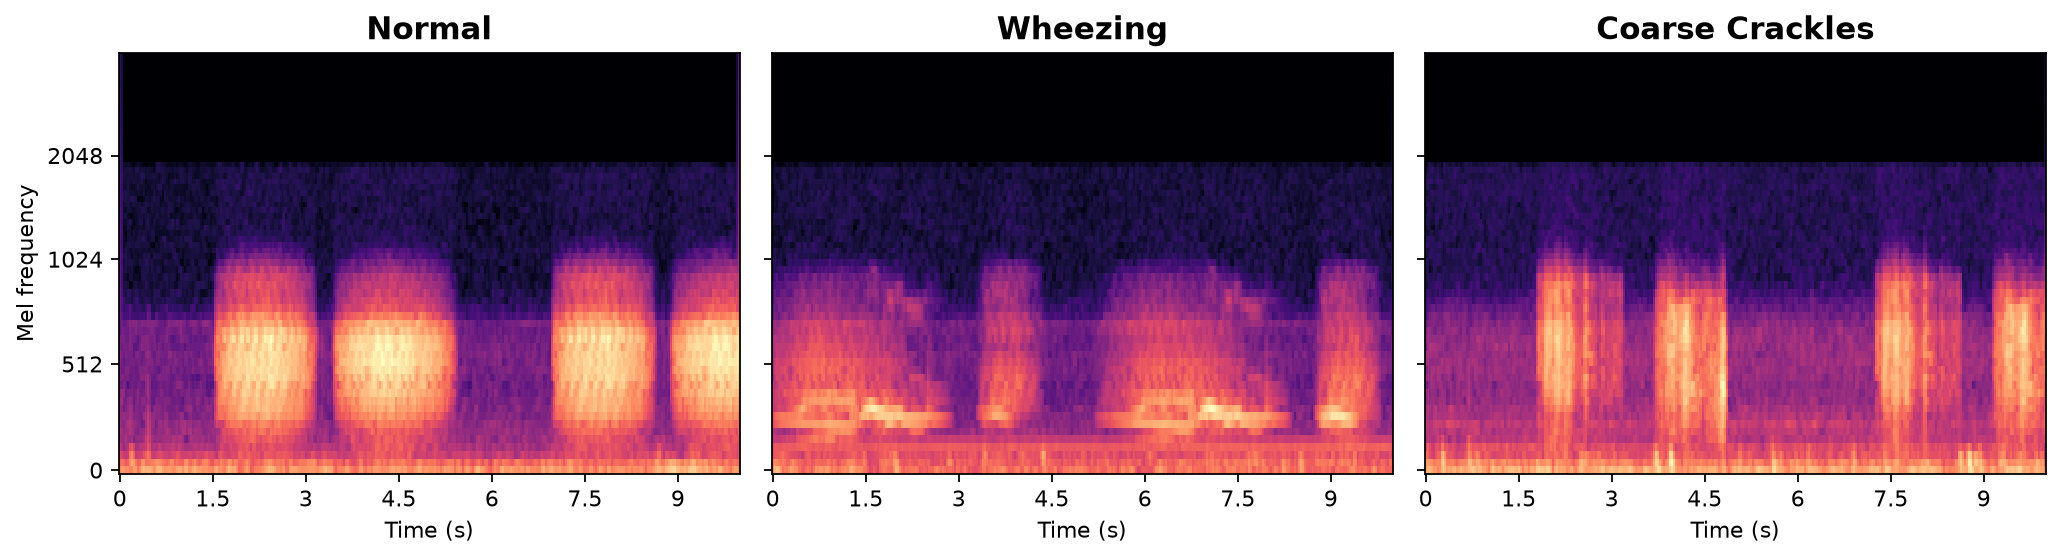
\includegraphics[width=0.70\textwidth]{figures/mel_spectrograms.png}}
{\fbox{\parbox[c][1.25in][c]{0.68\textwidth}{\centering Upload
\texttt{figures/mel\_spectrograms.png}.}}}}
\caption{Normalized log-mel spectrograms for three representative recordings.
Wheezing produces sustained horizontal bands corresponding to narrow-band
whistles, whereas coarse crackles appear as short vertical bursts distributed
across frequency. Normal breath sounds show smooth, broadband respiratory
cycles.}
\label{fig:spectrograms}
\end{figure*}

Two feature representations were derived from this common pipeline. For the MLP,
each spectrogram was reduced to the mean and standard deviation of every mel band
across time, producing a fixed 128-dimensional vector that summarizes the
spectral envelope and its temporal variability. Reducing 20{,}032 spectrogram
values to 128 features is substantial, and on a training set of 75 recordings
this compression acts as a strong structural prior. For the CNN, the complete
$1 \times 64 \times 313$ tensor was retained, preserving the local
time--frequency structure that a convolutional model is designed to exploit:
crackles and wheezes are defined by localized patterns rather than by average
spectral level.

% ---------------------------------------------------------------------------
% ORIGINAL heading -- INSERTED body
% ---------------------------------------------------------------------------
\section{Methodology}
This section describes the machine learning models and training procedure used
for the project.

\subsection{Model Architecture}
Two architectures were evaluated. The \textbf{multi-layer perceptron} was
implemented with scikit-learn's \texttt{MLPClassifier} \cite{b6} inside a
\texttt{Pipeline} containing a \texttt{StandardScaler}, so that feature
standardization is refit on each cross-validation training fold and never sees
held-out data. The best MLP used one hidden layer of 64 units with tanh activation. 
Counting the output layer, that comes to 8,646 trainable parameters.

The \textbf{convolutional neural network} was implemented in PyTorch \cite{b4} as
three convolutional blocks with channel widths 16, 32, and 64. Each block applies
a $3 \times 3$ convolution with padding of 1, batch normalization, and a ReLU
activation; the first two are followed by $2 \times 2$ max pooling and the third
by adaptive average pooling to a $1 \times 1$ extent. The result is flattened,
passed through a dropout layer, and mapped to six outputs by a linear layer,
giving 23{,}910 trainable parameters, nearly 3 times the MLP.

\subsection{Training Procedure}
Both models were trained on the 94 deduplicated recordings using stratified
splits, so each class remained roughly proportional across the train and test
sets. Without stratification, a small class such as the 13-example group could
be poorly represented in the test set. The MLP used a 20\% test split (75
training, 19 test), the CNN used a 25\% split (70 training, 24 test), and the
same random seed of 42 was used throughout for consistency.

Hyperparameters were tuned with \texttt{GridSearchCV} under stratified five-fold
cross-validation on the training partition, scored by accuracy. The search spaces
appear in Table~\ref{tab:grids}: 54 configurations (270 fits) for the MLP and 16
configurations (80 fits) for the CNN.

\begin{table}[htbp]
\caption{Hyperparameter Search Spaces}
\begin{center}
\begin{tabular}{ll}
\hline
\multicolumn{2}{c}{\textbf{MLP} (54 combinations)} \\
\hline
\texttt{hidden\_layer\_sizes} & (64,), (128,), (64, 32) \\
\texttt{activation} & relu, tanh, logistic \\
\texttt{alpha} & 1e-4, 1e-3, 1e-2 \\
\texttt{learning\_rate\_init} & 1e-3, 1e-2 \\
\hline
\multicolumn{2}{c}{\textbf{CNN} (16 combinations)} \\
\hline
\texttt{lr} & 1e-3, 1e-2 \\
\texttt{optimizer\_\_weight\_decay} & 1e-4, 1e-3 \\
\texttt{module\_\_dropout} & 0.30, 0.50 \\
\texttt{batch\_size} & 8, 16 \\
\hline
\end{tabular}
\label{tab:grids}
\end{center}
\end{table}

Three activation functions were compared for the MLP: the rectified linear unit,
the hyperbolic tangent, and the logistic sigmoid. 
The search selected \texttt{tanh} with a single 64-unit hidden layer,
$\alpha = 10^{-4}$, and an initial learning rate of $10^{-3}$, reaching a best
cross-validated accuracy of 0.880.

The CNN was trained with cross-entropy loss, and the network produced raw output values that were converted into class probabilities by the loss function.
Adam was used for optimization, with early stopping on a stratified
20\% internal validation split and a patience of 10 epochs, capped at 100 epochs.
To keep the comparison between models fair, the CNN was wrapped in a
skorch \cite{b7} \texttt{NeuralNetClassifier}, which exposes a scikit-learn
compatible interface, so the identical \texttt{GridSearchCV} and
\texttt{StratifiedKFold} procedure could be applied to both models over the same
folds with the same scoring rule. The selected CNN used a learning rate of
$10^{-3}$, weight decay of $10^{-4}$, dropout of 0.30, and a batch size of 8,
reaching a best cross-validated accuracy of 0.671.

% ---------------------------------------------------------------------------
% ORIGINAL list -- INSERTED justification paragraph
% ---------------------------------------------------------------------------
\subsection{Evaluation Metrics}
The trained models were evaluated using standard classification metrics:

\begin{itemize}
    \item accuracy;
    \item precision;
    \item recall;
    \item F1-score;
    \item confusion matrix.
\end{itemize}

Since the deduplicated classes are nearly balanced, accuracy can be deemed a suitable metric. 
If said classes were strongly skewed, accuracy would not be a reliable metric.
Accuracy alone is nonetheless insufficient. In single-label multi-class
classification, micro-averaged precision, recall, and F1 are numerically
identical to accuracy, so reporting them adds nothing. All figures in this
report are \emph{macro}-averaged, to give each class equal weight
regardless of size. Under macro averaging a class the model never predicts
contributes a zero rather than being absorbed by the remaining five, which proved
decisive in interpreting the CNN results.

% ---------------------------------------------------------------------------
% ORIGINAL heading -- INSERTED body, table filled
% ---------------------------------------------------------------------------
\section{Results}
Table~\ref{tab:model-results} compares the two models. Both were tuned by the
same grid-search procedure over the same cross-validation folds.

\begin{table}[htbp]
\caption{Model Performance Comparison}
\begin{center}
\begin{tabular}{lcc}
\hline
\textbf{Measure} & \textbf{MLP} & \textbf{CNN} \\
\hline
Cross-validated accuracy (grid search) & \textbf{0.880} & 0.671 \\
Held-out test accuracy & \textbf{0.84} & 0.75 \\
Macro precision & \textbf{0.88} & 0.66 \\
Macro recall & \textbf{0.83} & 0.72 \\
Macro F1-score & \textbf{0.82} & 0.68 \\
Trainable parameters & 8{,}646 & 23{,}910 \\
\hline
\end{tabular}
\label{tab:model-results}
\end{center}
\end{table}

The MLP outperforms the CNN on every metric. A separate five-fold
cross-validation of the tuned MLP over all 94 recordings gave per-fold accuracies
of 0.842, 0.842, 0.895, 0.895, and 0.778, averaging $0.850 \pm 0.043$. The small 
spread in these results suggests that the 0.84 test accuracy is fairly representative, 
rather than the result of a lucky split.

Fig.~\ref{fig:metric-comparison} shows the same comparison graphically. The gap
between the two models is wider under macro F1 (0.14) than under accuracy (0.09),
because macro averaging makes the CNN pay in full for a class it fails to predict
at all.

\begin{figure}[htbp]
\centerline{%
\IfFileExists{figures/metric_comparison.png}
{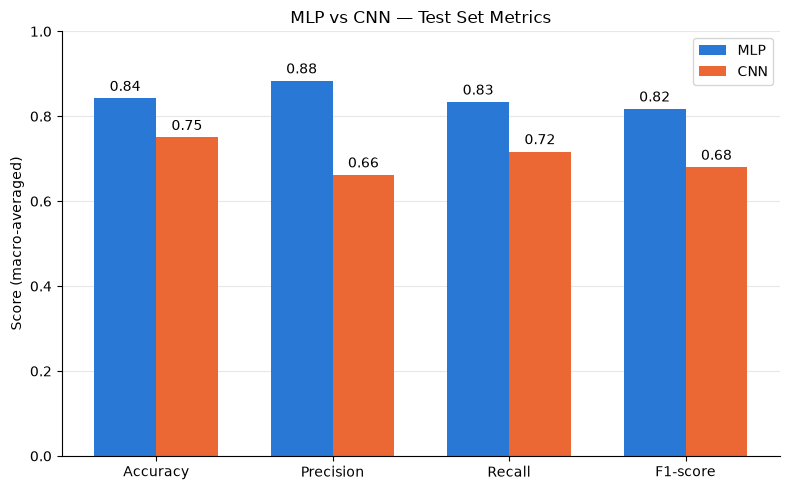
\includegraphics[width=0.82\columnwidth]{figures/metric_comparison.png}}
{\fbox{\parbox[c][1.25in][c]{0.8\columnwidth}{\centering Upload
\texttt{figures/metric\_comparison.png}.}}}}
\caption{Macro-averaged test-set metrics for the two models.}
\label{fig:metric-comparison}
\end{figure}

Per-class results are given in Table~\ref{tab:per-class}. Wheezing was recovered
perfectly by both models. Fine Crackles was the hardest class for both: the MLP
recovered one of three test clips, and the CNN never assigned the label to any
recording, producing precision, recall, and F1 of zero for that class.

\begin{table*}[htbp]
\caption{Per-Class Test-Set Performance}
\begin{center}
\begin{tabular}{lcccccccc}
\hline
& \multicolumn{4}{c}{\textbf{MLP}} & \multicolumn{4}{c}{\textbf{CNN}} \\
\textbf{Class} & \textbf{Precision} & \textbf{Recall} & \textbf{F1} &
\textbf{Support} & \textbf{Precision} & \textbf{Recall} & \textbf{F1} &
\textbf{Support} \\
\hline
Coarse Crackles & 0.75 & 1.00 & 0.86 & 3 & 0.60 & 0.75 & 0.67 & 4 \\
Fine Crackles & 1.00 & 0.33 & 0.50 & 3 & 0.00 & 0.00 & 0.00 & 3 \\
Normal & 1.00 & 0.67 & 0.80 & 3 & 1.00 & 0.75 & 0.86 & 4 \\
Pleural Rub & 0.80 & 1.00 & 0.89 & 4 & 0.57 & 0.80 & 0.67 & 5 \\
Rhonchi & 0.75 & 1.00 & 0.86 & 3 & 0.80 & 1.00 & 0.89 & 4 \\
Wheezing & 1.00 & 1.00 & 1.00 & 3 & 1.00 & 1.00 & 1.00 & 4 \\
\hline
\textbf{Macro average} & \textbf{0.88} & \textbf{0.83} & \textbf{0.82} &
\textbf{19} & \textbf{0.66} & \textbf{0.72} & \textbf{0.68} & \textbf{24} \\
\hline
\end{tabular}
\label{tab:per-class}
\end{center}
\end{table*}

The confusion matrices in Fig.~\ref{fig:confusion} show where the errors occur.
The MLP made three errors on 19 test recordings: two Fine Crackles clips were
labelled Coarse Crackles and Rhonchi respectively, and one Normal clip was
labelled Pleural Rub. The CNN made six errors on 24 recordings, and its errors
are more concentrated: Pleural Rub was predicted seven times for five true
instances, absorbing misclassified clips from three other classes.

\begin{figure*}[htbp]
\centerline{%
\IfFileExists{figures/mlp_confusion_matrix.png}
{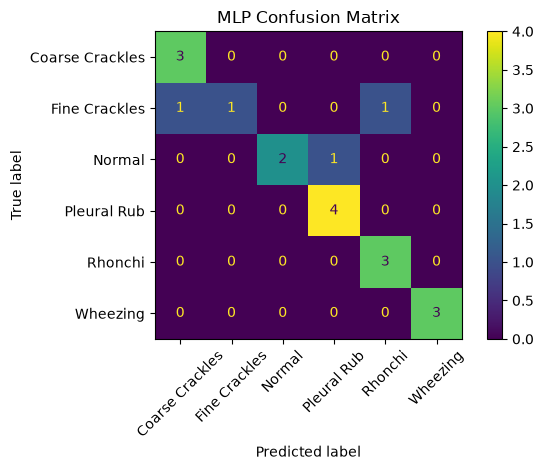
\includegraphics[width=0.33\textwidth]{figures/mlp_confusion_matrix.png}}
{\fbox{\parbox[c][1.25in][c]{0.32\textwidth}{\centering Upload
\texttt{figures/mlp\_confusion\_matrix.png}.}}}%
\hfil
\IfFileExists{figures/cnn_confusion_matrix.png}
{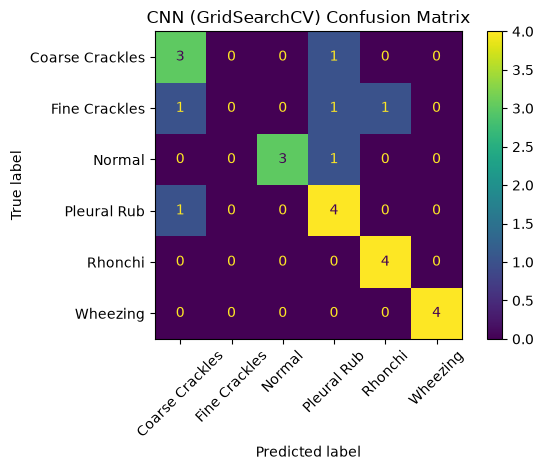
\includegraphics[width=0.33\textwidth]{figures/cnn_confusion_matrix.png}}
{\fbox{\parbox[c][1.25in][c]{0.32\textwidth}{\centering Upload
\texttt{figures/cnn\_confusion\_matrix.png}.}}}}
\caption{Confusion matrices on the held-out test sets: tuned MLP (left, 19
recordings) and tuned CNN (right, 24 recordings).}
\label{fig:confusion}
\end{figure*}

One result is not captured by any aggregate metric. Inspecting the Normal column
of both confusion matrices shows that every recording either model labelled
Normal was in fact Normal; no abnormal recording was ever classified as healthy.
The MLP's Normal recall of 0.67 reflects a Normal clip being flagged as Pleural
Rub, which for a screening application is the benign direction of error.

% ---------------------------------------------------------------------------
% ORIGINAL heading -- INSERTED body
% ---------------------------------------------------------------------------
\section{Discussion}
The MLP outperformed the CNN on every metric. A
likely explanation is that the dataset is very small. The CNN had to learn its
own feature detectors from only 70 training recordings, while the MLP was
trained on a simpler representation based on the mean and standard deviation of
each mel band. That made it easier for the MLP to perform well given the amount
of data available. This trade-off between model capacity and training set size
is a standard result in machine learning \cite{b1}.

The class-level results support this interpretation. Wheezing was easy for both
models, which is reasonable because wheezes appear as clear, sustained patterns
in the spectrogram. Crackles were much harder. They are short, low-energy
sounds, and the difference between coarse and fine crackles is subtle. For the
MLP, the averaging used to create the 128 features likely removed some of the
short-time details that define crackles. The CNN struggled even more, especially
with Fine Crackles, and it often assigned uncertain cases to Pleural Rub.

There is little evidence that the MLP was overfit. Its cross-validated accuracy
and its held-out test accuracy were very close, and the variation across folds
was relatively small. The CNN showed a larger gap between its cross-validated
and test accuracy, but with only 24 test recordings, that difference is still
small enough that it should not be overinterpreted.

\subsection{Class Balance and Resampling}
\label{sec:resampling}
A natural question is whether the small dataset could be improved with
resampling. After deduplication, the largest class has 18 recordings and the
smallest has 13, so the class imbalance is fairly mild. The bigger issue is not
imbalance alone, but the fact that there are simply not many examples overall.
Resampling and augmentation could still help, especially for the harder classes
such as Fine Crackles, but they are not a complete solution by themselves.

\textit{Oversampling in feature space:} Random oversampling duplicates
minority-class examples, while SMOTE \cite{b8} creates new examples by
interpolating between samples from the same class. This is straightforward for
the MLP because its input is already a fixed 128-dimensional vector. For the CNN,
though, the idea is less convincing because interpolating between two
spectrograms does not necessarily produce a realistic lung sound.

\textit{Undersampling:} Reducing every class to the size of the smallest would
leave 78 recordings and discard 16 of the 94 available. On a dataset this small,
that would probably remove useful information and hurt performance rather than
help it.

\textit{Audio-domain augmentation:} The most promising option is to augment the
data in the audio or spectrogram domain instead of the feature domain.
Label-preserving transformations such as time shifting, time stretching, pitch
shifting, adding background noise, and SpecAugment-style time and frequency
masking \cite{b10} can create new examples that still look like realistic
recordings. Because they are applied before feature extraction, they could help
both the CNN and the MLP. This is especially relevant for Fine Crackles, which
were the hardest class for both models.

A lighter alternative that does not create synthetic data is class weighting.
Both frameworks support it directly---\texttt{class\_weight} for scikit-learn
estimators and the \texttt{weight} argument to \texttt{CrossEntropyLoss} for the
CNN. This makes the model pay more attention to mistakes on minority classes
without duplicating or fabricating samples.

Whichever approach is used, one important rule should be followed: resampling
should happen inside the cross-validation loop and only on the training folds.
Applying SMOTE before the train/test split would let synthetic points derived
from test recordings leak into training, which would make the reported results
too optimistic. That is the same kind of problem as the duplicate recordings
discussed earlier, and it is easy to miss because the resampled data still looks
well formed. The \texttt{imbalanced-learn} pipeline \cite{b9} can combine
resampling with an estimator in a way that is safe for cross-validation.

Any gain from these methods would also need to be judged carefully. With only
three to five test recordings per class, a single correctly or incorrectly
classified clip can change recall by 0.20 to 0.33. To show a real improvement,
we would need repeated or nested cross-validation rather than a single held-out
split.

\subsection{Limitations}
Several limitations affect how strong these conclusions are.

\begin{itemize}
    \item \textbf{Dataset size.} Ninety-four recordings is very small. A test
    split of 19 to 24 clips means that one recording can change the accuracy by
    several points, so small differences between models are not very meaningful.
    \item \textbf{Single held-out split.} The test results come from one
    stratified split. The cross-validated results ($0.850 \pm 0.043$ for the MLP)
    are a more reliable estimate of generalization.
    \item \textbf{Ordering sensitivity.} The file index is built by globbing
    directories, so the order of the files determines which copy of a duplicate
    pair is kept. An earlier run of the same code selected a two-layer $(64,
    32)$ architecture instead of the $(64,)$ architecture reported here. Sorting
    the file list before deduplication would remove this variation.
    \item \textbf{No patient-level grouping.} Recordings are split at random, so
    two recordings from the same subject could end up on opposite sides of the
    split. Grouped cross-validation would be stricter and more clinically
    realistic.
    \item \textbf{Limited hyperparameter search.} The CNN grid covered 16
    configurations and varied no architectural parameters beyond dropout. Filter
    counts, kernel sizes, and depth were fixed.
\end{itemize}

% ---------------------------------------------------------------------------
% ORIGINAL heading -- INSERTED body
% ---------------------------------------------------------------------------
\section{Conclusion}

This project builds a pipeline that classifies lung sound recordings into six
categories. When creating this pipeline, cleaning and deduplicating the dataset
proved to be very critical to ensure that the model was not memorizing the data.
Of the 195 initial files, 101 were exact duplicates, leaving only 94 recordings.
Had this step not been caught, accuracy would have looked deceptively high.

Our best MLP reached 0.880 cross-validated accuracy and 0.84 on the test set,
with a macro F1 of 0.82. The CNN, tuned the same way, reached 0.671 and 0.75,
with a macro F1 of 0.68. Of the three activations we tried, tanh worked best.
Initial guesses led towards the CNN performing better due to spectrograms
mirroring image classification, but the MLP overall outperformed the CNN, likely
due to the 70 training recordings being too small to learn on.

In the future, to address this problem, we would use augmentation, which is
oversampling done on the audio rather than on the features. Fine Crackles is the
obvious place to start, since neither model handled it well and there are only 13
recordings of it. We should also have run that experiment instead of only
reasoning about it.



\begin{thebibliography}{00}
% --- ORIGINAL entries [1]-[4] -- unchanged ---
\bibitem{b1} I. Goodfellow, Y. Bengio, and A. Courville, \textit{Deep Learning}.
Cambridge, MA, USA: MIT Press, 2016.

\bibitem{b2} B. McFee et al., ``librosa: Audio and music signal analysis in
Python,'' in \textit{Proc. 14th Python in Science Conf.}, 2015, pp. 18--25.

\bibitem{b4} A. Paszke et al., ``PyTorch: An imperative style, high-performance
deep learning library,'' in \textit{Advances in Neural Information Processing
Systems}, vol. 32, 2019.

% --- INSERTED entries [5]-[10] ---
\bibitem{b5} ``HLS-CMDS dataset,'' IEEE DataPort, 2025. [Online]. Available:
\url{https://doi.org/10.1109/IEEEDATA.2025.3566012}

\bibitem{b6} F. Pedregosa et al., ``Scikit-learn: Machine learning in Python,''
\textit{J. Mach. Learn. Res.}, vol. 12, pp. 2825--2830, 2011.

\bibitem{b7} skorch Developers, ``skorch: A scikit-learn compatible neural
network library that wraps PyTorch,'' 2017. [Online]. Available:
\url{https://skorch.readthedocs.io}

\bibitem{b8} N. V. Chawla et al., ``SMOTE: Synthetic minority over-sampling
technique,'' \textit{J. Artif. Intell. Res.}, vol. 16, pp. 321--357, 2002.

\bibitem{b9} G. Lema\^{i}tre, F. Nogueira, and C. K. Aridas,
``Imbalanced-learn: A Python toolbox to tackle imbalanced datasets in machine
learning,'' \textit{J. Mach. Learn. Res.}, vol. 18, no. 17, pp. 1--5, 2017.

\bibitem{b10} D. S. Park et al., ``SpecAugment: A simple data augmentation
method for automatic speech recognition,'' in \textit{Proc. Interspeech}, 2019,
pp. 2613--2617.
\end{thebibliography}

\end{document}
